% This is the Reed College LaTeX thesis template. Most of the work
% for the document class was done by Sam Noble (SN), as well as this
% template. Later comments etc. by Ben Salzberg (BTS). Additional
% restructuring and APA support by Jess Youngberg (JY).
% Your comments and suggestions are more than welcome; please email
% them to cus@reed.edu
%
% See https://www.reed.edu/cis/help/LaTeX/index.html for help. There are a
% great bunch of help pages there, with notes on
% getting started, bibtex, etc. Go there and read it if you're not
% already familiar with LaTeX.
%
% Any line that starts with a percent symbol is a comment.
% They won't show up in the document, and are useful for notes
% to yourself and explaining commands.
% Commenting also removes a line from the document;
% very handy for troubleshooting problems. -BTS

% As far as I know, this follows the requirements laid out in
% the 2002-2003 Senior Handbook. Ask a librarian to check the
% document before binding. -SN

%%%%%%%%%%%%%%%%%%%%%%%%%%%%%%%%%%%%%%%%%%%%%%%%%%%%%%%%%%%%%%%%%%%%%%%%%%%%%%%%
%%%%%%%%%%%%%%%%%%%%%%%%%%%%%%%%% Preamble %%%%%%%%%%%%%%%%%%%%%%%%%%%%%%%%%%%%%
%%%%%%%%%%%%%%%%%%%%%%%%%%%%%%%%%%%%%%%%%%%%%%%%%%%%%%%%%%%%%%%%%%%%%%%%%%%%%%%%

\documentclass[12pt,oneside]{ucrthesis}
\usepackage{graphicx,latexsym}
\usepackage{amsmath}
\usepackage{amssymb,amsthm}
\usepackage{longtable,booktabs,setspace}
\usepackage{setspace} \doublespacing
\usepackage[hyphens]{url}
\usepackage[hidelinks]{hyperref}
\usepackage{lmodern}
\usepackage{float}
\usepackage{lipsum}
\floatplacement{figure}{H}
\usepackage{calc}
\usepackage{rotating}
\usepackage{biblatex}
\setlength\bibitemsep{\baselineskip} % Creates one line of space between entries
\usepackage{lscape}


\renewcommand{\hyperref}[2][???]{\autoref{#1}}
\def\chapterautorefname{Chapter}
\def\sectionautorefname{Section}
\def\subsectionautorefname{Subsection}

\usepackage{caption}
\captionsetup{width=5in}

\usepackage{palatino} % other fonts are available like times, bookman, charter, palatino


%% Siunitx for common and custom SI units
\usepackage{siunitx}
\DeclareSIUnit\molar{\mole\per\cubic\deci\metre}
\DeclareSIUnit\Molar{\textsc{M}}
\DeclareSIUnit\nt{\textsc{nt}}
\DeclareSIUnit\units{\textsc{U}}

\newcommand{\beginsupplement}{%
        \setcounter{table}{0}
        \renewcommand{\thetable}{S\arabic{table}}%
        \setcounter{figure}{0}
        \renewcommand{\thefigure}{S\arabic{figure}}%
     }

% To pass between YAML and LaTeX the dollar signs are added by CII
\title{This is my title}
\author{Troy R. Alva}
\date{Month Year}
\division{Bourns College of Engineering}
\advisor{Dr.~PI}
\institution{University of California}
\degree{Doctor of Philosophy}
\department{Major}
\degreemonth{Month}
\degreeyear{year}
\degreesemester{quarter}
\othermembertwo{Dr.~Committee 1}
\othermemberthree{Dr.~Committee 2}
\campus{Riverside}
\doctype{Dissertation}

%%% Copied from knitr
%% maxwidth is the original width if it's less than linewidth
%% otherwise use linewidth (to make sure the graphics do not exceed the margin)
\makeatletter
\def\maxwidth{ %
  \ifdim\Gin@nat@width>\linewidth
    \linewidth
  \else
    \Gin@nat@width
  \fi
}
\makeatother

% From {rticles}
\newlength{\csllabelwidth}
\setlength{\csllabelwidth}{3em}
\newlength{\cslhangindent}
\setlength{\cslhangindent}{1.5em}
% for Pandoc 2.8 to 2.10.1
\newenvironment{cslreferences}%
  {}%
  {\par}
% For Pandoc 2.11+
% As noted by @mirh [2] is needed instead of [3] for 2.12
\newenvironment{CSLReferences}[2] % #1 hanging-ident, #2 entry spacing
 {% don't indent paragraphs
  \setlength{\parindent}{0pt}
  % turn on hanging indent if param 1 is 1
  \ifodd #1 \everypar{\setlength{\hangindent}{\cslhangindent}}\ignorespaces\fi
  % set entry spacing
  \ifnum #2 > 0
  \setlength{\parskip}{#2\baselineskip}
  \fi
 }%
 {}
\usepackage{calc} % for calculating minipage widths
\newcommand{\CSLBlock}[1]{#1\hfill\break}
\newcommand{\CSLLeftMargin}[1]{\parbox[t]{\csllabelwidth}{#1}}
\newcommand{\CSLRightInline}[1]{\parbox[t]{\linewidth - \csllabelwidth}{#1}}
\newcommand{\CSLIndent}[1]{\hspace{\cslhangindent}#1}

\renewcommand{\contentsname}{Table of Contents}
% End of CII addition

\setlength{\parskip}{0pt}

% Added by CII

\providecommand{\tightlist}{%
  \setlength{\itemsep}{0pt}\setlength{\parskip}{0pt}}

\Acknowledgements{\lipsum}

\Dedication{\lipsum}

\Abstract{\lipsum}

	\usepackage[width=\textwidth]{caption}
 \captionsetup[figure]{font=footnotesize}
 \captionsetup[table]{font=footnotesize}
 \newcommand{\blandscape}{\begin{landscape}}
 \newcommand{\elandscape}{\end{landscape}}
% End of CII addition
%%
%% End Preamble
%%
%
\begin{document}

\maketitle

\frontmatter
% \pagestyle{empty}
\begin{acknowledgements}
  \lipsum
\end{acknowledgements}
\begin{dedication}
  \begin{center}
    \null\vfil
    \lipsum
    \null\vfil
  \end{center}
\end{dedication}
\begin{abstract}
  \begin{center}
  \begin{singlespace}
    ABSTRACT OF THE \expandafter\uppercase\expandafter{Dissertation}\par
    \vspace{.5in}
    This is my title\par
    \vspace{.25in}
    by\par
    \vspace{.25in}
    Troy R. Alva\par
    \vspace{.25in}
    Doctor of Philosophy, Graduate Program in Major\par
    University of California, Riverside, Month year\par
    Dr.~PI, Chairperson\par
    \vspace{.25in}
  \end{singlespace}
  \end{center}
      \lipsum
\end{abstract}

\hypersetup{linkcolor=black}
\setcounter{secnumdepth}{2}
\setcounter{tocdepth}{2}

% \begin{singlespace}
\tableofcontents

\cleardoublepage
% \phantomsection
\addcontentsline{toc}{chapter}{\listfigurename}
\listoffigures

\cleardoublepage
% \phantomsection
\addcontentsline{toc}{chapter}{\listtablename}
\listoftables
% \end{singlespace}


\mainmatter % here the regular arabic numbering starts
\pagestyle{fancyplain} % turns page numbering back on

\hypertarget{introduction}{%
\chapter*{Introduction}\label{introduction}}
\addcontentsline{toc}{chapter}{Introduction}

\markright{Introduction}

This is how you cite a reference in dissertation.bib.
Let's cite Troy R. Alva, (Alva et al., 2021)

\lipsum

\hypertarget{chapter1-tag}{%
\chapter{Chapter 1 title}\label{chapter1-tag}}

\lipsum

\hypertarget{introduction-1}{%
\section{Introduction}\label{introduction-1}}

\lipsum

\hypertarget{materials-and-methods}{%
\section{Materials and Methods}\label{materials-and-methods}}

\lipsum

\hypertarget{results}{%
\section{Results}\label{results}}

\lipsum

\hypertarget{discussion}{%
\section{Discussion}\label{discussion}}

\lipsum

\hypertarget{chapter2-tag}{%
\chapter{Chapter 2 title}\label{chapter2-tag}}

\lipsum

\hypertarget{introduction-2}{%
\section{Introduction}\label{introduction-2}}

\lipsum

\hypertarget{materials-and-methods-1}{%
\section{Materials and Methods}\label{materials-and-methods-1}}

\lipsum

\hypertarget{results-1}{%
\section{Results}\label{results-1}}

\lipsum
\begin{landscape}






\begin{figure}[h]

{\centering 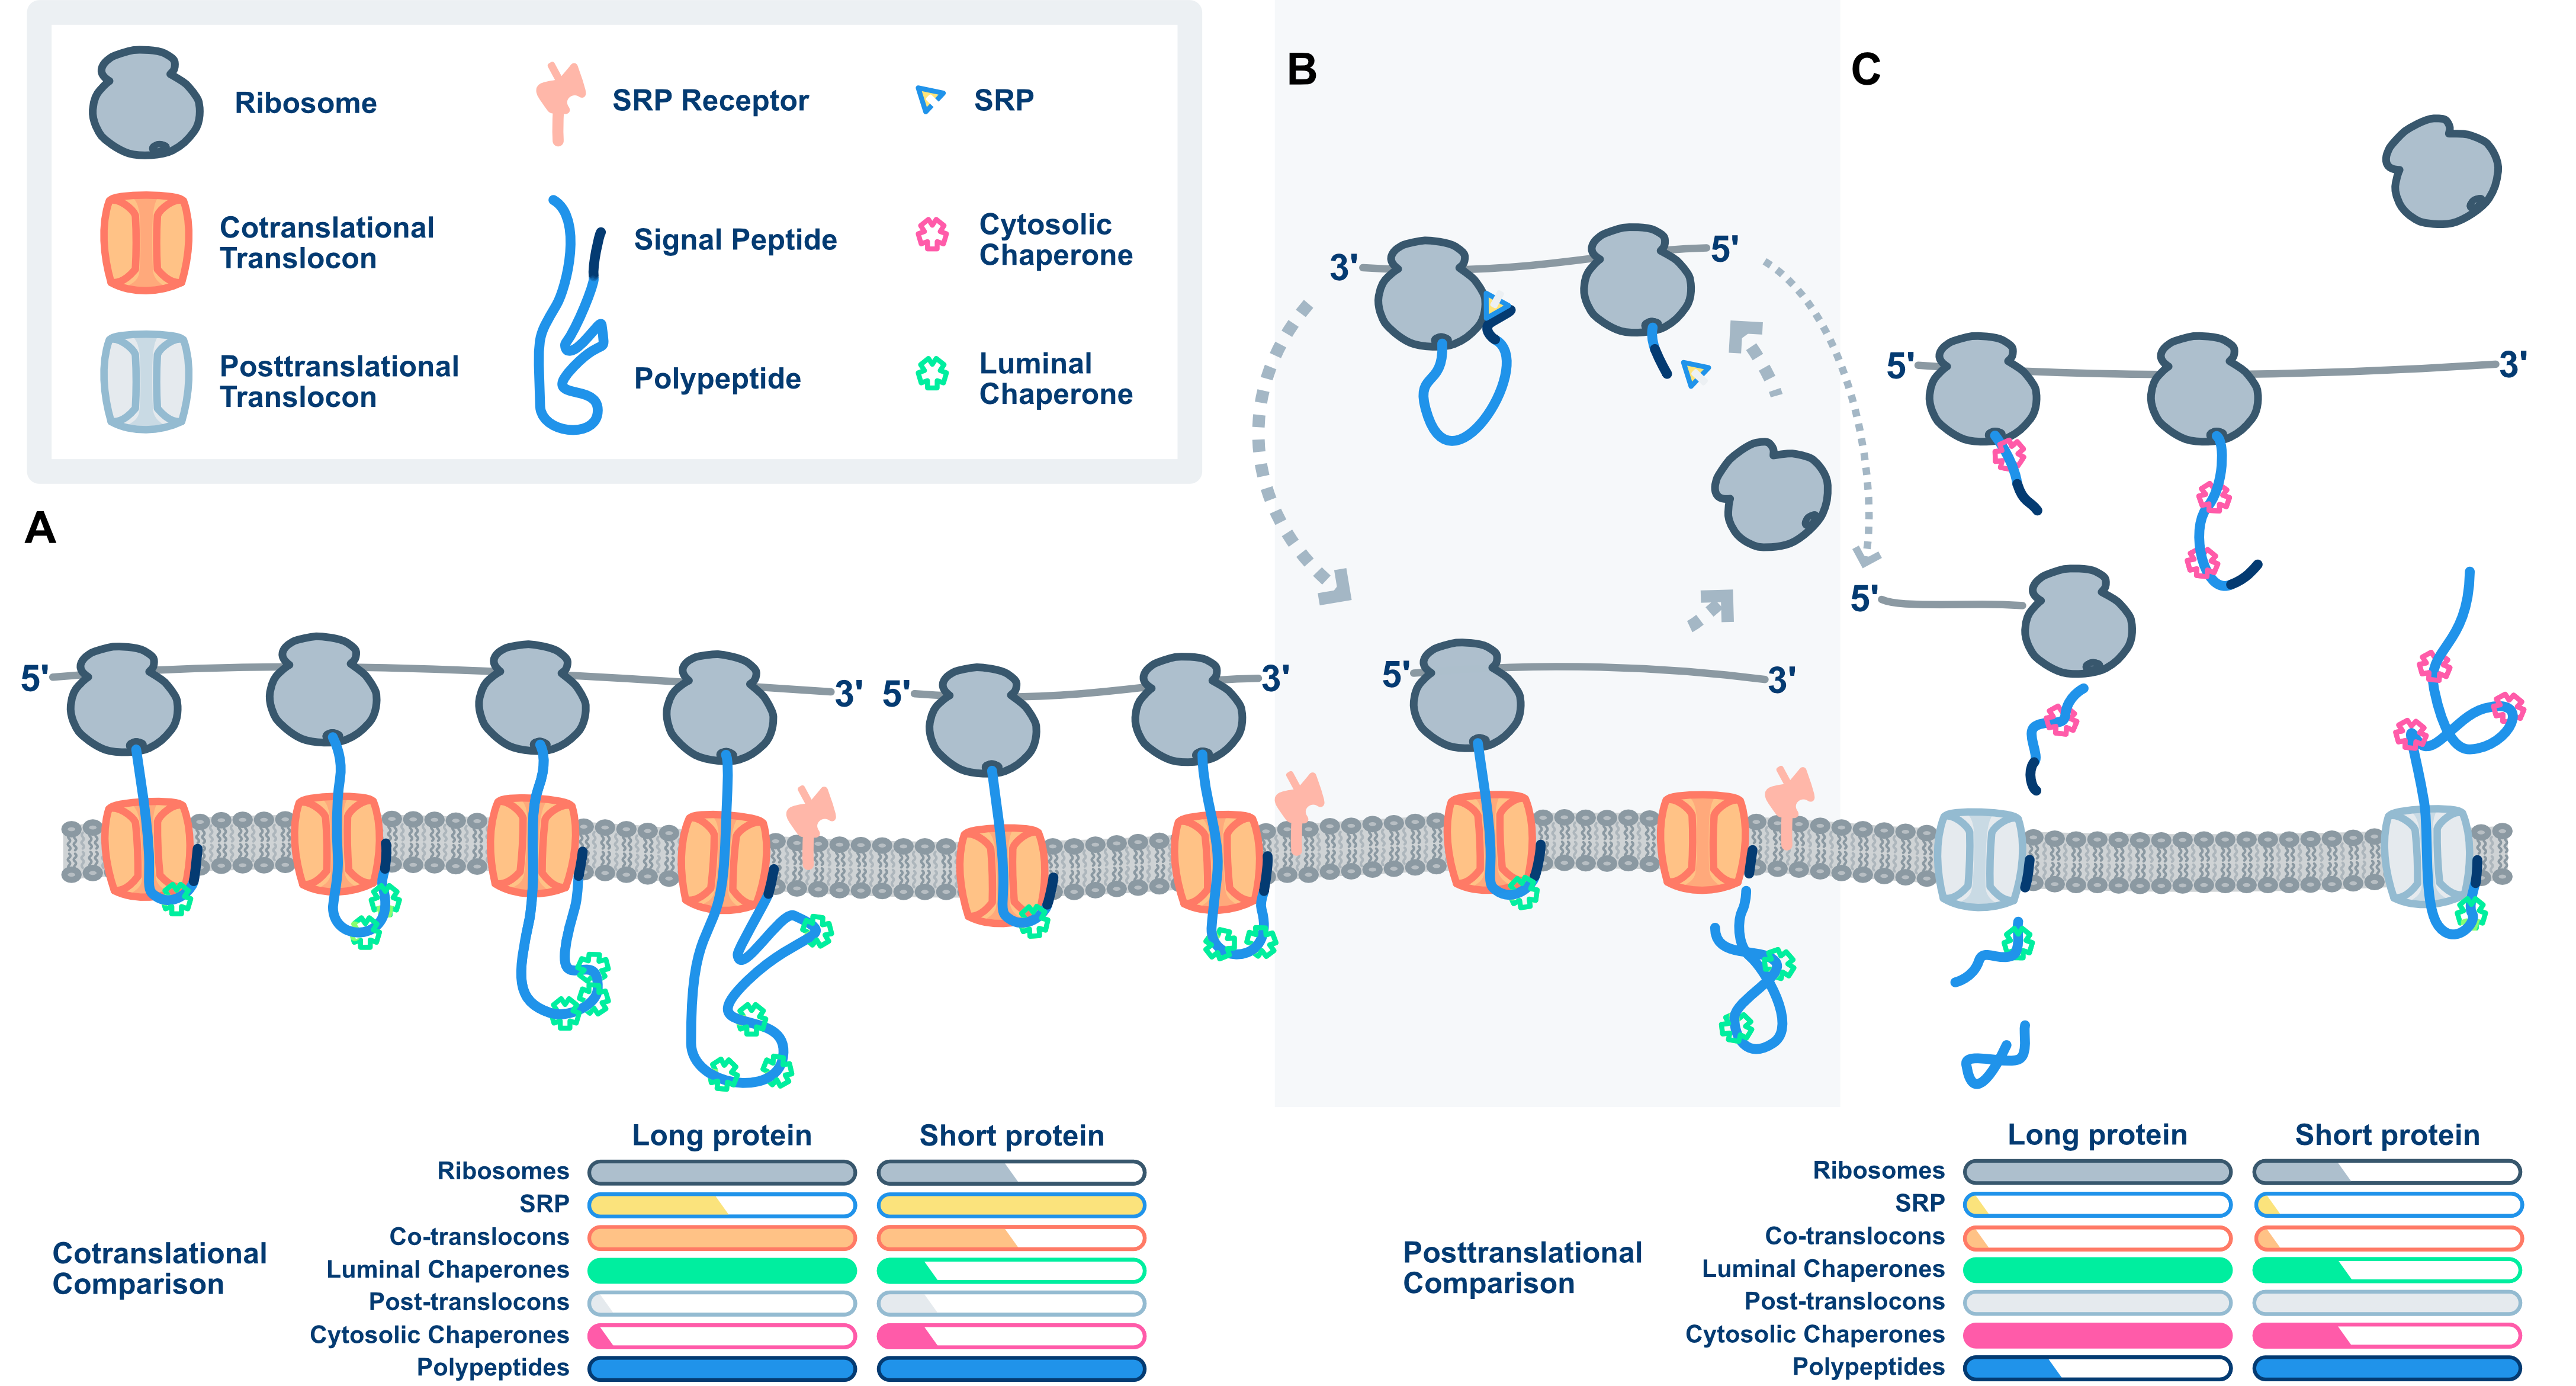
\includegraphics[width=1\linewidth]{images/expression_metrics} 

}

\caption[This is a short caption for list of figures]{\textbf{Example caption for figure}
\textbf{\emph{a}} Describes plot subsection.
\textbf{\emph{b}} Describes plot subsection.
\textbf{\emph{c}} Describes plot subsection.}\label{fig:metrics}
\end{figure}
\end{landscape}
\hypertarget{discussion-1}{%
\section{Discussion}\label{discussion-1}}

\lipsum

\hypertarget{chapter3-tag}{%
\chapter{Chapter 3 title}\label{chapter3-tag}}

\lipsum

\hypertarget{introduction-3}{%
\section{Introduction}\label{introduction-3}}

\lipsum

\hypertarget{materials-and-methods-2}{%
\section{Materials and Methods}\label{materials-and-methods-2}}

\lipsum

\hypertarget{results-2}{%
\section{Results}\label{results-2}}

\lipsum






\begin{figure}[h]

{\centering 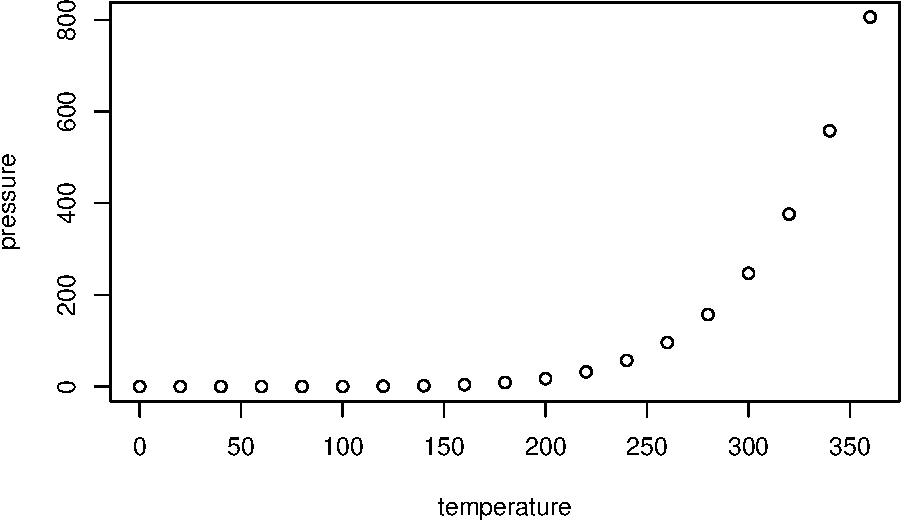
\includegraphics[width=1\linewidth]{dissertation_files/figure-latex/scatter-1} 

}

\caption[This is a short caption for list of figures]{\textbf{Example caption for figure}
\textbf{\emph{a}} Describes plot subsection.
\textbf{\emph{b}} Describes plot subsection.
\textbf{\emph{c}} Describes plot subsection.}\label{fig:scatter}
\end{figure}
\hypertarget{discussion-2}{%
\section{Discussion}\label{discussion-2}}

\lipsum

\hypertarget{conclusion}{%
\chapter*{Conclusion}\label{conclusion}}
\addcontentsline{toc}{chapter}{Conclusion}

\markright{Conclusion}

\lipsum

\backmatter
\singlespace
\setlength{\parindent}{-0.20in}
\setlength{\leftskip}{0.20in}
\setlength{\parskip}{8pt}

\hypertarget{references}{%
\chapter*{References}\label{references}}
\addcontentsline{toc}{chapter}{References}

\markboth{References}{References}

\hypertarget{refs}{}
\begin{CSLReferences}{1}{0}
\leavevmode\vadjust pre{\hypertarget{ref-troy_alva-mc}{}}%
(7) ({PDF}) efficient facemask sterilization via forced ozone convection, n.d.

\leavevmode\vadjust pre{\hypertarget{ref-Alva2021-qo}{}}%
Alva, T.R., Riera, M., Chartron, J.W., 2021. Translational landscape and protein biogenesis demands of the early secretory pathway in komagataella phaffii. Microb. Cell Fact. 20, 19.

\end{CSLReferences}
\noindent

\hypertarget{section}{%
\section{}\label{section}}

nocite: \textbar{}
{``(7) ({PDF}) efficient facemask sterilization via forced ozone convection''} (n.d.)
\ldots{}

\hypertarget{appendix}{%
\chapter*{Appendix}\label{appendix}}
\addcontentsline{toc}{chapter}{Appendix}


% Index?

\end{document}
